\documentclass[10pt, conference, compsocconf]{IEEEtran}

\usepackage{capt-of}
\usepackage{graphicx}
\usepackage{subfig}
\usepackage{booktabs}
\usepackage{multirow}
\usepackage{siunitx}
\usepackage{multicol}
\usepackage{array}
\usepackage{amsmath}
\newcommand{\BIBdecl}{\setlength{\itemsep}{0.0 em}}


\newcommand{\nltable}[2][c]{%
  \begin{tabular}[#1]{@{}c@{}}#2\end{tabular}}
\newcommand{\wave}{\raise.17ex\hbox{$\scriptstyle\mathtt{\sim}$}}

\newcolumntype{C}[1]{>{\centering\let\newline\\\arraybackslash}m{#1}}

\begin{document}
\bstctlcite{IEEEexample:BSTcontrol}

\title{Distributed Matrix Multiplication Performance Estimator \\for Machine Learning Jobs in Cloud Computing}
%  Remark: Please note that most journals do not allow the use of abbreviations in titles. Please check the target journal guidelines to verify the same and revise accordingly.

\author{\IEEEauthorblockN{Myungjun Son}
\IEEEauthorblockA{Department of Computer Science\\
Kookmin University\\
Seoul, South Korea\\
smj8612@kookmin.ac.kr}
\and
\IEEEauthorblockN{Kyungyong Lee}
\IEEEauthorblockA{Department of Computer Science\\
Kookmin University\\
Seoul, South Korea\\
leeky@kookmin.ac.kr}
}

% make the title area
\maketitle

\begin{abstract}
  Matrix multiplication is an important kernel task in many machine learning algorithms. As the size of input datasets increases, multiple workloads are analyzed in large-scale distributed cloud computing environments. Therefore, understanding the characteristics of a distributed matrix multiplication task is essential for running machine learning jobs in the cloud. Herein, we propose Matrix multiplication Performance Estimator for Cloud computing (\textbf{MPEC}), a method to predict the latency of matrix multiplication of various sizes and shapes in a distributed cloud computing environment. We first characterize the overhead of a distributed matrix multiplication task and propose features to model the latency of a task with different input types. Using the proposed features, a latency prediction model is developed by applying a data mining algorithm and a parameter optimization step iteratively. In experiments with 236 distinct types of matrix multiplications on diverse cloud instances running Apache Spark, we confirm that the proposed method can model the latency of various types of matrix multiplication tasks effectively and capture the non-linear interactions among the proposed features. A comparison with the state-of-the-art cloud computing performance predictor reveals that MPEC provides 16\% greater accuracy for a distributed matrix multiplication task and confirms the uniqueness of the distributed matrix multiplication workload.
\end{abstract}

\IEEEpeerreviewmaketitle

\section{Introduction}\label{sec:intro}
Many big data analysis systems are deployed in cloud computing environments to process increasingly large datasets while guaranteeing stable operations, scalability, and fault-tolerance from the viewpoint of infrastructure. To satisfy application demands from distinct use cases, cloud computing service providers offer various types of configuration instances, and many big data systems are deployed in a scale-out manner using cloud computing resources. In such environments, managing distributed compute resources, datasets, and programming is challenging. To relieve the burden of managing distributed resources and allow application developers to focus on critical tasks, many systems that provide simple and easy interfaces to handle large-scale datasets have been proposed, e.g., Apache Spark~\cite{spark}.

Data mining algorithms are used to extract valuable information from massive datasets, and in many machine learning algorithms, matrix multiplication is the core computation kernel. For example, in recommendation systems, the core computation kernel of matrix factorization algorithms, such as SVD and NMF~\cite{nmf}, is matrix-matrix multiplication. Matrix-vector multiplication is the core kernel of the PageRank algorithm when using the power method to obtain principle eigenvectors~\cite{pagerank}. To build a cost-efficient cloud environment wherein machine learning tasks can be performed with a distributed matrix computation kernel, it is crucial to estimate the overhead of kernel tasks with distinct matrix sizes and shapes.

To understand the characteristics of matrix multiplication performance in a distributed cloud computing environment, we analyzed the performance of dense matrix multiplication with diverse input sizes and formations on distinct cloud computing instances. In the experiments, we multiplied two square matrices(10000, 20000, and 30000 rows) on AWS EC2 \textit{R4, C4}, and \textit{G2} instances with a size of \textit{2xlarge}. We used the Apache Spark MLlib BlockMatrix library~\cite{spark-mm} to conduct the experiments with four machines with OpenBLAS installed.

\begin{figure}[t]
  \centering
  \subfloat[Different instance types]{\label{fig:different-instance-types}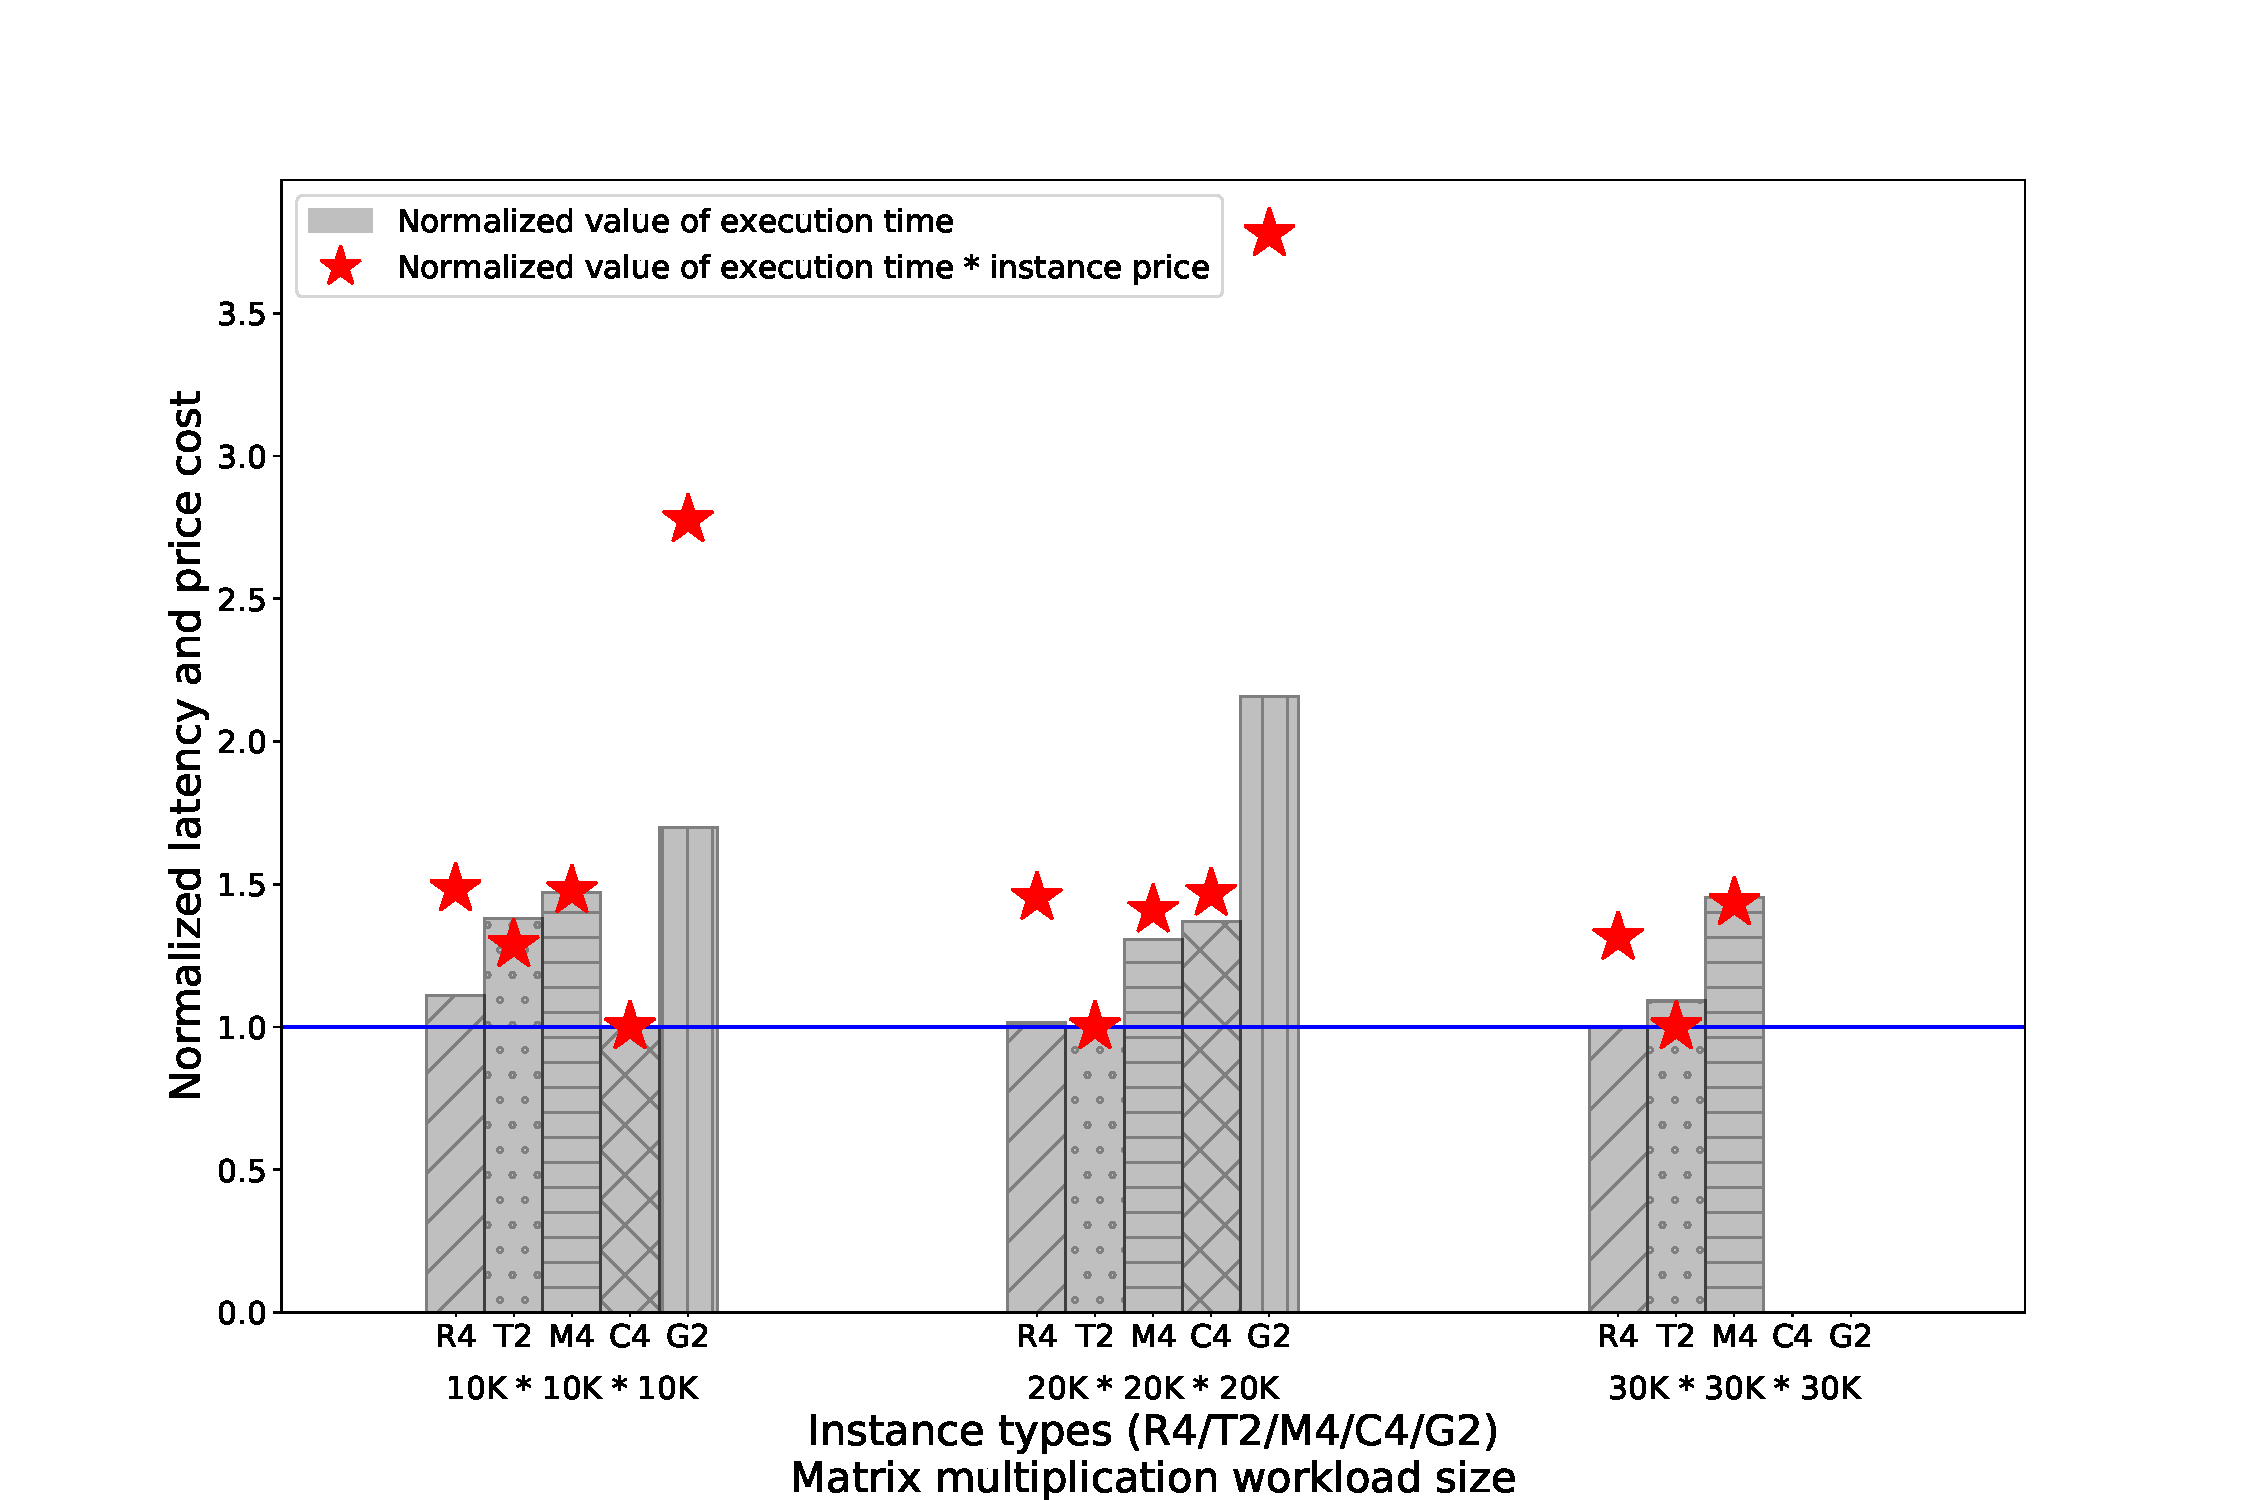
\includegraphics[width=4.5cm,height=4.5cm]{figures/instance-2xl-compare.pdf}}\hfil\hfil\hfil\hfil\hfil\hfil\hfil\hfil\hfil\hfil\subfloat[Different matrix shapes]{\label{fig:different-matrix-shapes}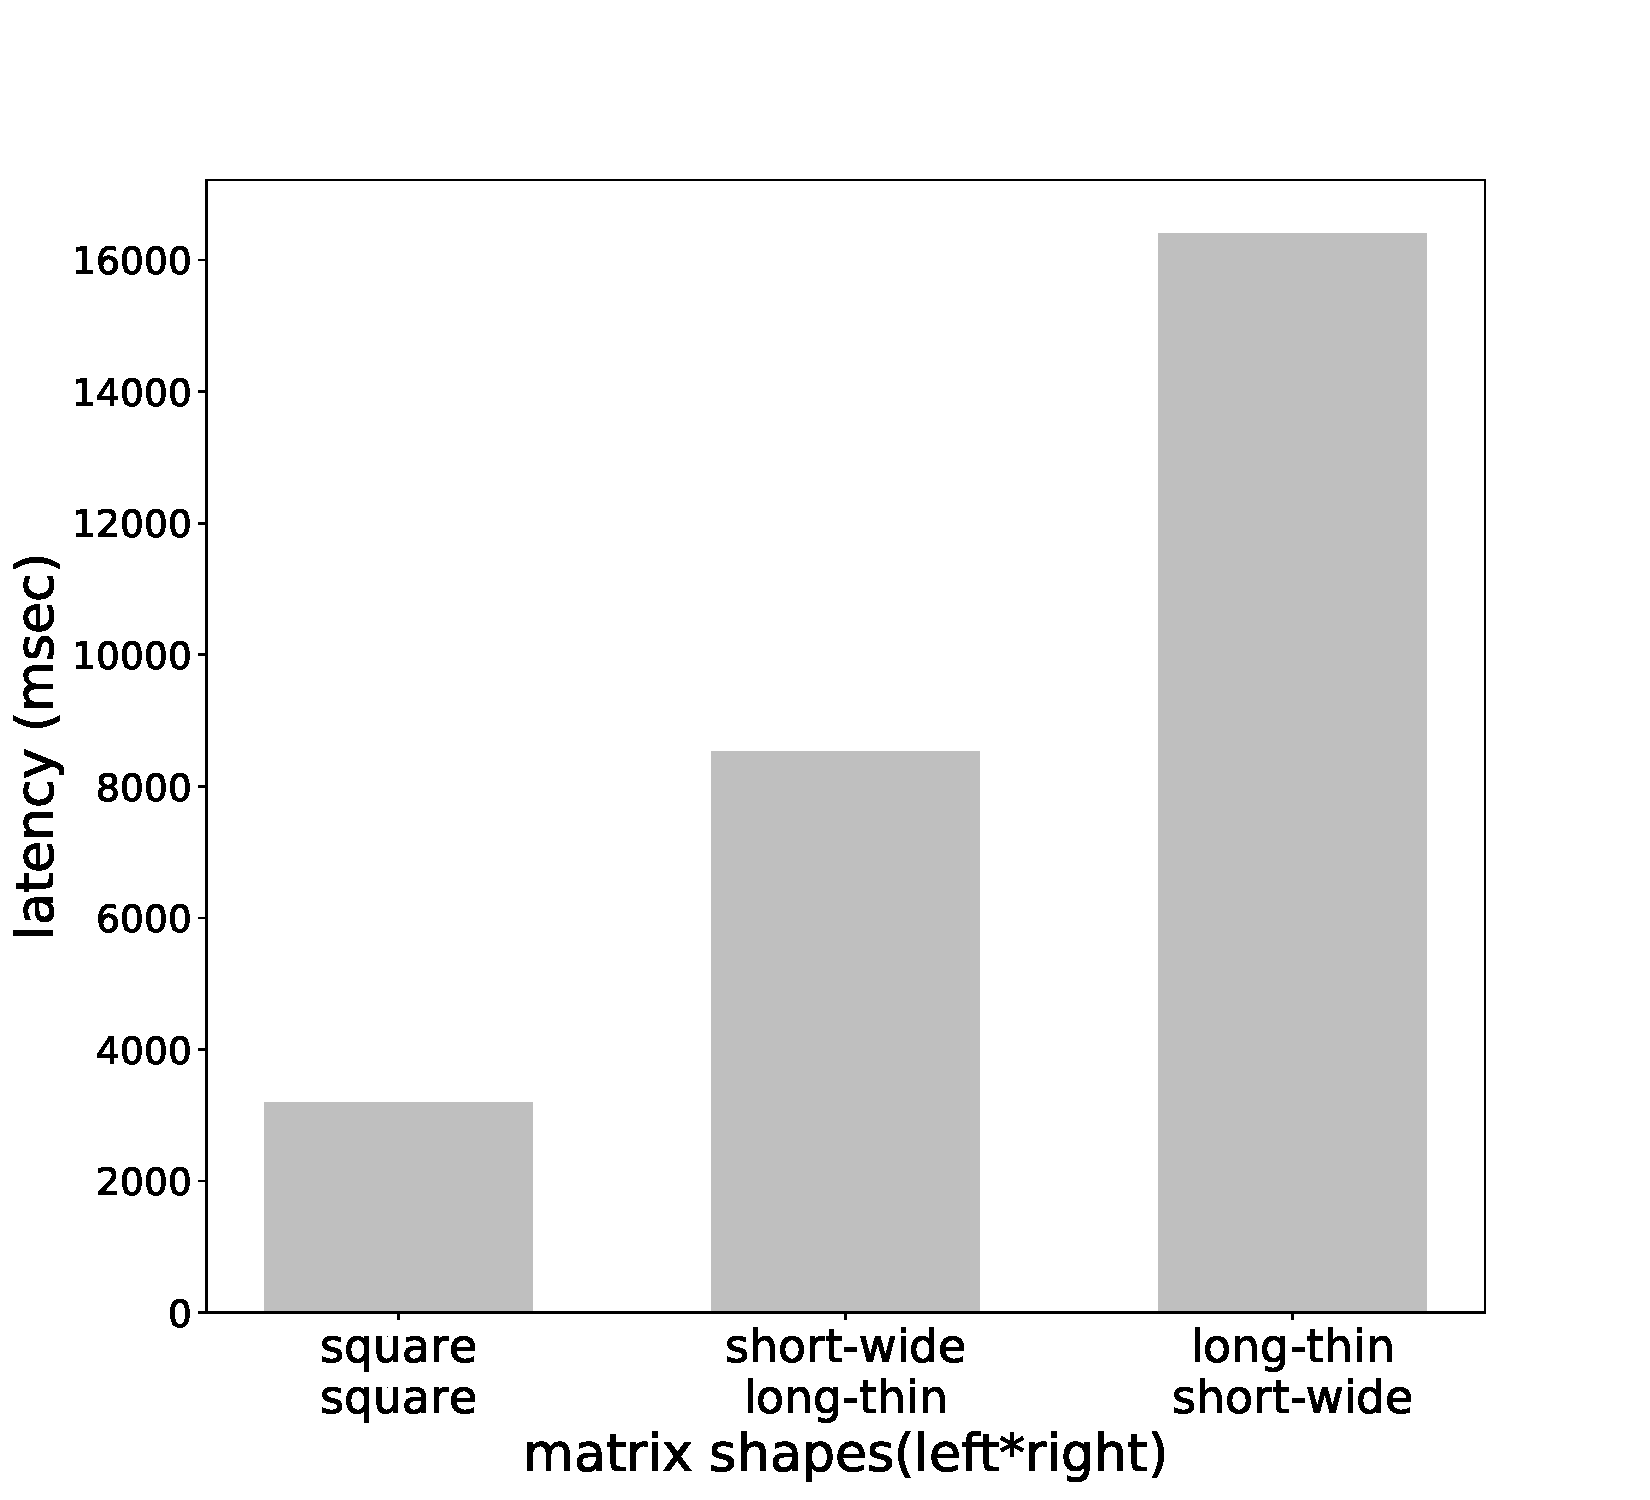
\includegraphics[width=4cm, height=4.5cm]{figures/matrix-multiplication-different-shape.pdf}}
  \caption{\label{fig:instance-blocks-sizes-compare}Normalized value of latency with different instance types and input matrix shapes (lower values are better)}
\end{figure}

In Figure~\ref{fig:different-instance-types}, the gray bar indicates the normalized latency of the fastest completing instance type. As shown in the figure, when the input matrix size differs, the best performing instance type differs. If we consider the price of each instance, the performance difference increases further (red star). Furthermore, as shown in Figure~\ref{fig:different-matrix-shapes}, the multiplication of two non-square matrices exhibits significantly different performance in comparison with that of square matrix multiplication even when the number of multiplication operations is the same, i.e., the number of left matrix rows $\times$ left matrix columns $\times$ right matrix columns. From the results shown in Figure~\ref{fig:instance-blocks-sizes-compare}, it is evident that estimating the latency of distributed matrix multiplication tasks with different matrix sizes and shapes is challenging.

Despite the importance of matrix multiplication in machine learning, comprehensive performance analyses and modeling in a distributed cloud computing environment have not been undertaken. Some methods, e.g., Ernest~\cite{ernest}, CherryPick~\cite{cherrypick}, and PARIS~\cite{paris}  focus on predicting machine learning task performance in a cloud computing environment. These methods rely on scale-based sampling to estimate the latency to complete a task with the entire original input dataset and show sufficient accuracy for some machine learning tasks. However, they show poor accuracy for predicting the latency of distributed matrix multiplication tasks because they fail to capture the complexity of the task. Many studies have investigated performance optimization, modeling, and prediction on a single machine with multiple cores using hardware-optimized libraries, e.g., OpenBLAS. However, these studies did not consider network and I/O overhead, which can be significant in a distributed cloud computing environment.

In this paper, we propose Matrix multiplication Performance Estimator for Cloud computing (MPEC), a method to predict the latency of matrix multiplication of arbitrary shapes and sizes using various cloud computing resource configurations. To represent the characteristics of distributed matrix multiplication tasks, such as the total number of multiplication operations, shuffle overhead, and output matrix size, the proposed MPEC employs eight features for modeling the task latency of distributed matrix multiplication. A prediction model is built using a gradient boosting (GB) regressor, followed by Bayesian optimization to find optimal hyper-parameters. The experimental results from more than 200 diverse matrix sizes and shapes demonstrate that MPEC can predict performance latency with a prediction error less than 16\%. Furthermore, a comparison of MPEC to Ernest~\cite{ernest}, a state-of-the-art machine learning cloud computing task performance evaluator, demonstrates that MPEC is 16\% more accurate at predicting the distributed matrix multiplication task latency.

The primary contributions of this study are as follows:
\begin{itemize}
  \item{Characterizing distributed matrix multiplication}
  \item{Proposing unique features to effectively represent distributed matrix multiplication tasks overheads}
  \item{Uncovering the non-linearity among features, and proposing latency prediction model}
  \item{Uncovering GPU cloud instances do not provide efficient distributed matrix multiplication operations}
\end{itemize}
%clarify as to what is being modeled

\begin{figure}[ht]
	\centering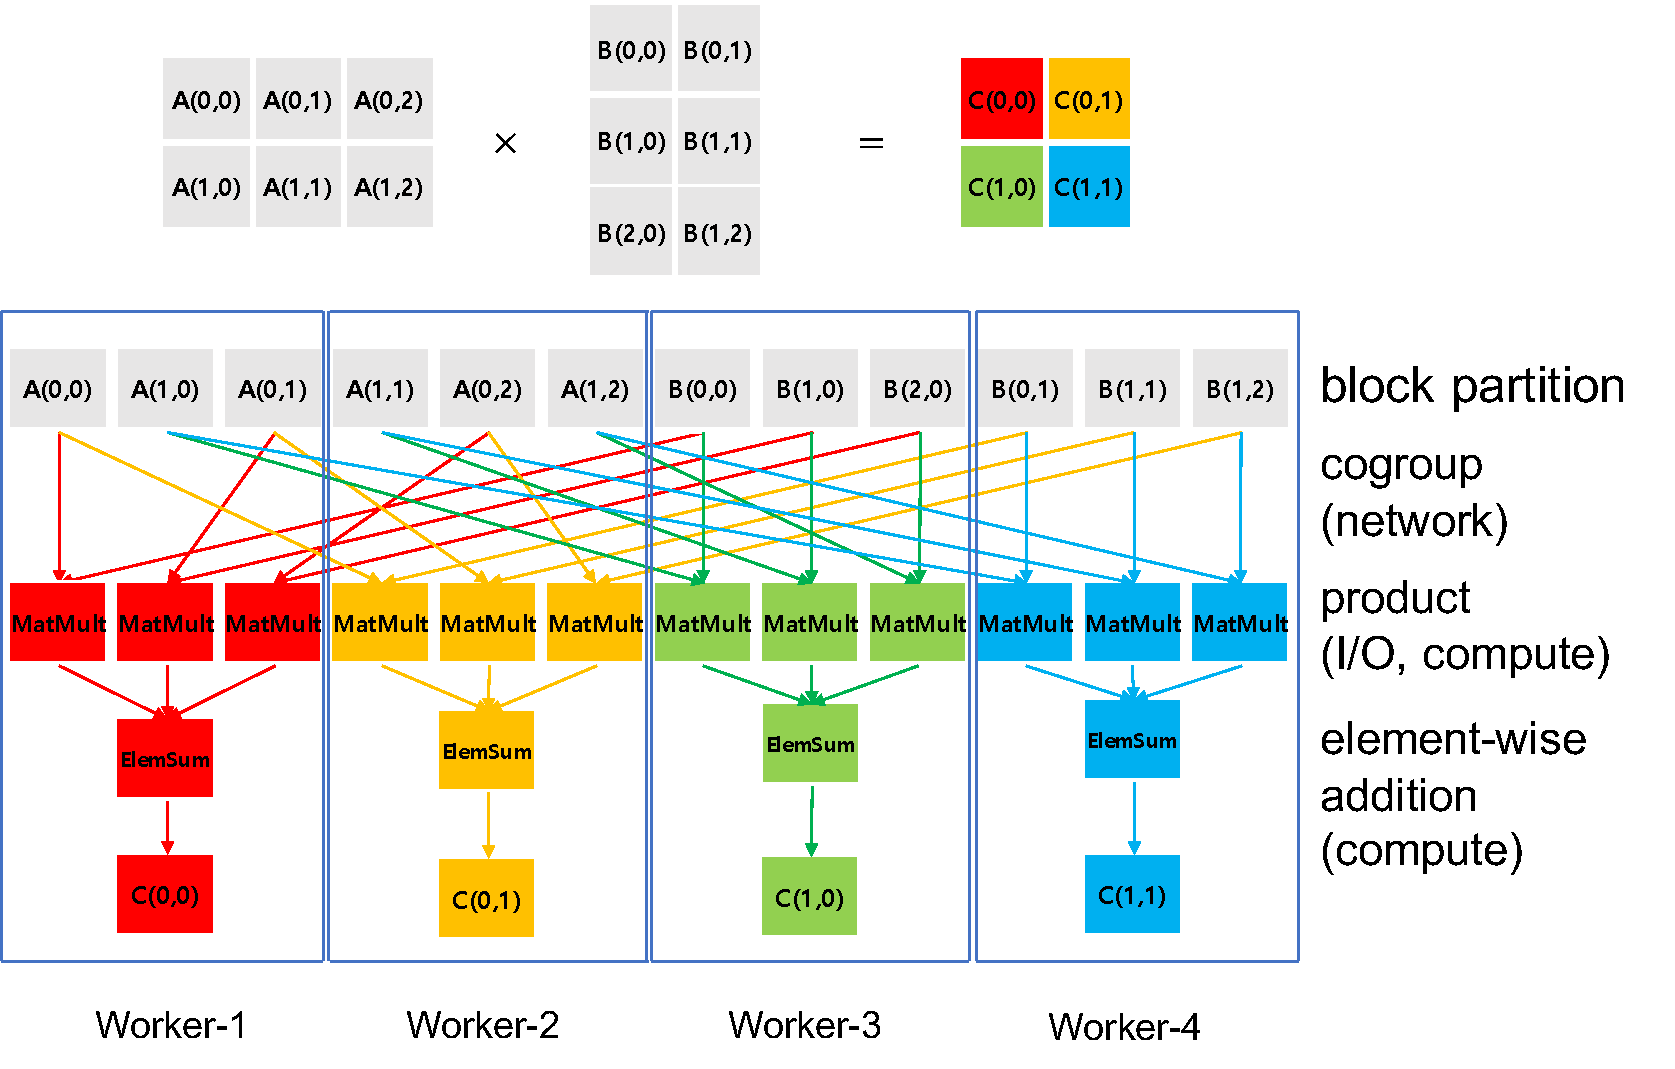
\includegraphics[width=0.5\textwidth]{figures/matmult-overhead-non-square-1.pdf}\caption{Block-based distributed matrix multiplication and related overhead in each step. Network, I/O, and CPU are the principal resources of the execution.}\label{fig:matmul-with-overhead}
\end{figure}

\section{Matrix Multiplication in Distributed Computing Environments}\label{sec:distributed-matrix-computation}
The optimization of distributed matrix multiplication has been well studied in the literature. In the HPC community, many studies have focused on minimizing the communication cost using the MPI model. The representative methods include SUMMA~\cite{summa} and CARMA~\cite{carma}. These methods demonstrate optimal performance with respect to minimizing communication costs; however, they have limitations in terms of programmability, scalability, and robustness in comparison with general-purpose big data analysis systems, e.g., Spark~\cite{spark}, particularly in shared cloud computing environments.

Apache Spark is an open source big data analysis platform. The primary abstraction in Spark is a Resilient Distributed Dataset, which represents a read-only collection of objects partitioned across a set of machines. Spark manages large-scale data using partitions that help to parallelize distributed data processing while guaranteeing fault tolerance with lineage and task execution optimization via lazy evaluation ~\cite{spark}.

In Spark, matrix-related linear algebraic operations are supported in the MLlib library~\cite{spark-mm} with various matrix-partitioning schemes (row-, column-, and block-based) and a set of distributed operation APIs on the matrix. To multiply two matrices, Spark MLlib automatically identifies the optimal way of task distribution based on the input matrix-partitioning scheme and uses the Scala Breeze library to perform multiplication. Consider $C = A \times B$, i.e., the multiplication of two matrices. If $A$ is row-partitioned and $B$ is column-partitioned, the Cartesian product is performed for each row block of $A$ and column block of $B$. If both $A$ and $B$ are block-partitioned, the block dimension of the resulting matrix $C$ is determined by considering the number of worker nodes and input block dimensions. A worker node that is responsible for each resulting block fetches all the necessary blocks from $A$ and $B$ to execute a multiplication operation locally.


Figure~\ref{fig:matmul-with-overhead} shows an example of block-based matrix multiplication. Here, the left matrix $A$, right matrix $B$, and the result matrix $C$ are  $2 \times 3$,  $3 \times 2$, and $2 \times 2$ block matrices, respectively. In Spark, a \textit{cogroup} operation allows a worker node, responsible for the result block, to collect the necessary left and right matrix blocks by block IDs. During a \textit{cogroup} operation, network overhead is dominant. After collecting all necessary blocks, each worker node performs product operations, followed by element-wise addition operations. In this step, the I/O overhead to read the fetched blocks from a \textit{local.dir} location and the compute overhead are dominant.

\subsection{Modeling the  Distributed Matrix Multiplication Overhead }\label{sec:overhead-modeling}
Dense matrix multiplication is a CPU-intensive task; however, other resource overheads become non-negligible when dense matrix multiplication is executed in a large-scale distributed computing environment, e.g., Spark. To qualitatively understand the characteristics of a distributed matrix multiplication task, we summarize the I/O, network, and compute overheads. Here, $LR$ and $LC$ are the number of rows and columns of a left matrix, respectively, and  $RC$ is the number of columns of a right matrix. Thus, the size of the resulting matrix is $LR \times RC$. Note that the left, right, and the resulting matrices are block-partitioned, and block sizes are denoted by $lr$, $lc$, and $rc$, where $LR \geq lr$, $LC \geq lc$, and $RC \geq rc$.

\textbf{Shuffle}: A worker node responsible for computing an output matrix block of size $lr \times rc$ must fetch blocks from the left and right matrices of size  $lr \times LC$ and $LC \times rc$, respectively. If the required blocks are unavailable locally, the worker node must fetch them from remote machines, which involves network overhead. Assuming uniform block distributions among worker nodes, the network overhead in the shuffle phase can be expressed as follows:
%Equation~\ref{eq:shuffle-overhead}.
\begin{equation}\label{eq:shuffle-overhead}
  BlockFetchOverhead_{lr \times rc} \propto \sum\limits_{i=1}^{\frac{LC}{lc}} lr \times lc + lc \times rc
\end{equation}

\textbf{Compute}: After a shuffle step is complete, the worker node performs multiplication on the fetched blocks, followed by element-wise addition. To perform multiplication, the blocks must be read from Spark's local directory (\textit{spark.local.dir} configuration), which is generally set as a disk storage device. Thus, the I/O read overhead is the same as the shuffle overhead and can be computed using Equation~\ref{eq:shuffle-overhead}.

After loading the input matrix blocks into memory, each worker node executes a multiplication task. Here, the overhead is expressed as follows. Equation~\ref{eq:compute-overhead}.
\begin{equation}\label{eq:compute-overhead}
  ComputeOverhead_{lr \times rc} \propto \sum\limits_{i=1}^{\frac{LC}{lc}} lr \times lc \times rc
\end{equation}

In the element-wise addition, the number of addition operations for each cell is proportional to $\frac{LC}{lc}$, and the size of each output block is $lr \times rc$.

\section{Matrix Multiplication Performance Estimation}\label{sec:mpc-structure}The proposed MPEC attempts to predict the latency involved in multiplying dense matrices of different sizes and shapes. As matrix multiplication is a core kernel task in many machine learning algorithms for big data analytics, we attempt to predict the matrix multiplication performance for various cloud computing resources wherein many recent big data systems are deployed.
% resource or instances ?
\begin{figure}
  \centering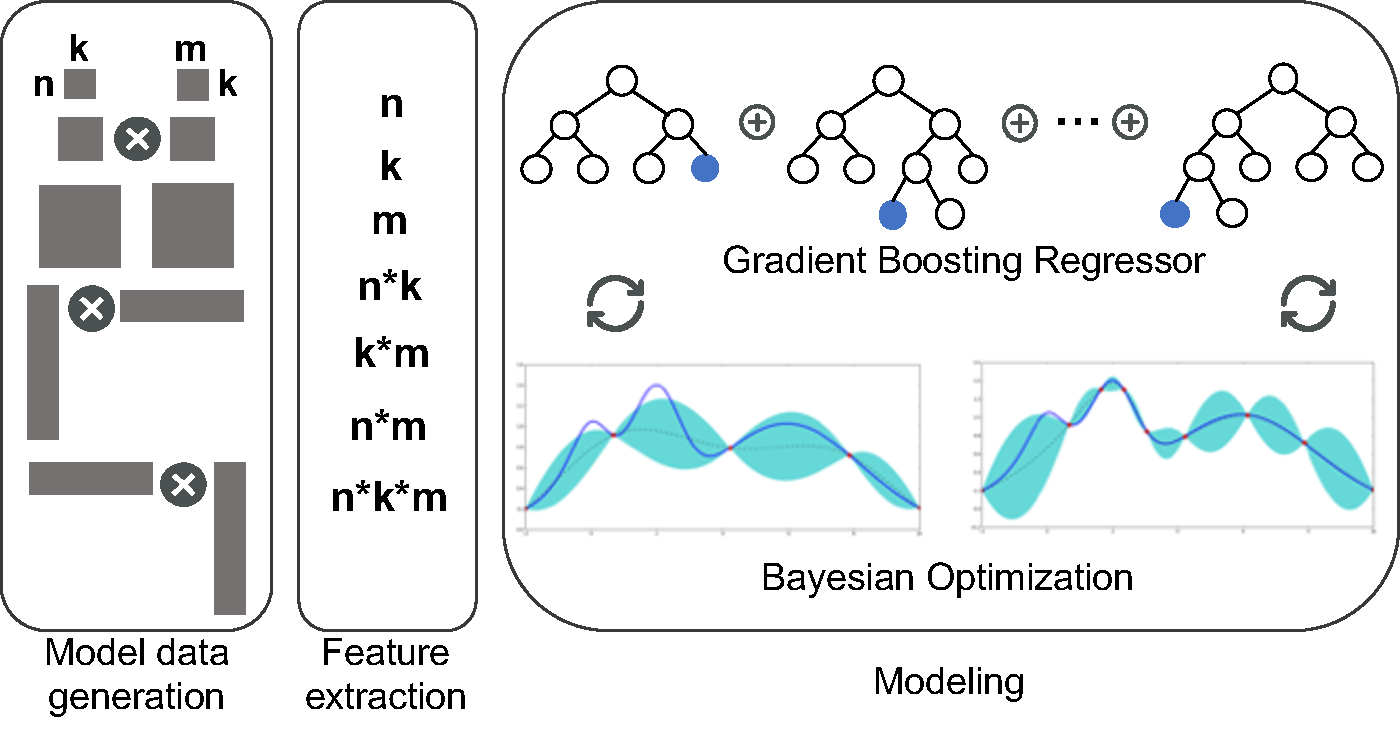
\includegraphics[width=0.5\textwidth]{figures/mpc-architecture.pdf}\caption{MPEC architecture}\label{fig:mpc-architecture}
\end{figure}

The MPEC architecture, which comprises tasks of training dataset generation, feature extraction, and modeling, is shown in Figure~\ref{fig:mpc-architecture}. In the modeling step, we perform Bayesian optimization~\cite{bayesian-optimization} iteratively to find the optimal working hyper-parameters of the selected modeling algorithm.

\subsection{Training Data Generation}\label{sec:train-data}
In the training dataset generation step, the MPEC performs offline profiling of various shapes and sizes of matrix multiplication to construct a model for predicting the latency of an arbitrary input dataset. Matrix multiplication tasks can be broadly categorized as  square $\times$ square, long-thin $\times$ short-wide, and short-wide $\times$ long-thin tasks. To cover all shapes and sizes, the MPEC profiles the latency of synthetically generated left and right matrices. In the latency measurement, the MPEC utilizes the Apache Spark web UI REST API, which provides various execution metrics in the JSON format.

To obtain optimal performance for various cloud computing instances with distinct capacity, MPEC adopts OpenBLAS for performing computation on a CPU and NVBLAS to compute instances that employ GPU devices~\cite{NVBLAS}. Note that we use netlib-java~\cite{fatman-littleboy} for allowing Spark to interact with hardware-optimized linear algebra libraries.

\subsection{Feature Extraction}\label{sec:features}
As discussed in Section~\ref{sec:overhead-modeling}, the matrix multiplication overhead in a distributed computing environment involves various resources. To account for such diverse overheads, MPEC utilizes the dimensions and products of input matrix blocks, i.e., $lr$, $lc$, $rc$, $lr \times rc$, $lr \times lc$, $lc \times rc$, $lr \times lc + lc \times rc$, and $lr \times lc \times rc$, as features to model the matrix multiplication performance. Here, the $lr \times rc$ term represents the size of the output matrix, the $lr \times lc$ and $lc \times rc$ terms represent the size of the left and right matrix blocks, respectively, where the size impacts the network and I/O disk overheads. The $lr \times lc \times rc$ term represents the total number of multiply operations.

Unlike MPEC, previous methods focus on predicting the performance of data mining tasks on cloud computing resources using a scale-based sampling mechanism as an input feature for prediction~\cite{cherrypick, ernest, paris}. Generally, these methods select a considerably small portion of the input dataset and measure performance using a subset of the dataset. Using the outcomes from the sample dataset, these methods apply distinct predictive algorithms, e.g., a non-negative linear equation (Ernest), Bayesian optimization (Cherrypick), and random forest (PARIS), to make a prediction. However, the scale-based sampling mechanism cannot capture the complex nature of distributed matrix multiplication and it considers either $lr$ or $rc$ based on the sampling method. Accordingly, the proposed MPEC demonstrates superior performance owing to its rich set of features (Section~\ref{sec:eval}).

\subsection{Modeling}\label{sec:modeling}
In the modeling step, the proposed MPEC builds a model to represent the performance of multiplying various matrices. This step comprises  model construction and hyper-parameter search. MPEC utilizes GB regressor~\cite{gradient-boosting} for the model construction step and Bayesian optimization~\cite{bayesian-optimization} to find optimal parameters for the GB method.

GB~\cite{gradient-boosting} is a flexible non-parametric statistical learning approach for classification and regression. The main idea behind GB is combining multiple weak learners that are generally applicable to only simple linear relations incrementally in order to model complex and non-linear interactions among features. A GB model is fitted in a forward stage-wise pattern, where at each stage, a new weak learner model is fitted to the residual of the current model, and the model focuses more on correcting errors from the previous iterations. Unlike a similar decision tree method, the GB method is robust against overfitting as it creates an ensemble of many weak learner models~\cite{random-forest}.

When building a predictive model, appropriately setting the model parameters is crucial for improving the prediction quality. Many heuristic methods, e.g., random walk, grid-based search, and adoption of statistical inference, have been proposed for searching the best performing hyper-parameters. The proposed MPEC utilizes a statistical inference method based on the Bayesian model~\cite{bayesian-optimization}. The Bayesian optimization method searches for a set of next configuration values that are likely to improve the model quality or reduce uncertainty. This is a non-parametric black box approach that estimates an objective function (i.e., the complete performance measure from all parameter combinations) using a stochastic process, e.g., a Gaussian process. When predicting the objective function, Bayesian optimization uses all information available from previous runs ($prior$) and the objective function model is updated ($posterior$) after new experiments are conducted ($likelihood$).

\section{Evaluation}{\label{sec:eval}}
We evaluate the performance of the proposed MPEC thoroughly using various types of cloud computing instances, input matrix sizes, and shapes. In summary, applying the GB algorithm with the proposed features outperforms a linear regressor and exhibits  42\% greater prediction accuracy. Furthermore, by applying Bayesian optimization to the selection of GB hyper-parameters, we could improve the prediction accuracy by approximately 2\%. An evaluation of the MPEC with various types of cloud instances demonstrates its effectiveness in a cloud computing environment. Finally, a comparison of MPEC with Ernest~\cite{ernest}, a state-of-the-art machine learning performance predictor for cloud computing, indicates that MPEC exhibits approximately 16\% better accuracy when predicting matrix multiplication latency.

\subsection{Setup}
To create diverse matrix multiplication scenarios for this evaluation, we generate left and right matrices with different numbers of rows and columns (128 - 8,000,000). Within this range, we generate 236 synthetic test cases of square $\times$ square, long-thin $\times$ short-wide, and short-wide $\times$ long-thin matrices\footnote{Test input cases - http://bit.ly/2CvOmnK}. Matrix multiplication is performed using Apache Spark and the MLlib library (version 2.2.0). Multiplication of each matrix size is executed five times, and the median value is used to represent the latency of the task. Unless otherwise stated, a Spark cluster is deployed to AWS EC2 using the \textit{spark-ec2} library\footnote{https://github.com/kmu-leeky/spark-ec2} with four \textit{R4.2xlarge} instances. Each EC2 instance has a hardware-optimized linear algebra library installed, i.e., NVBLAS for GPU instances (\textit{g2.2xlarge}) and OpenBLAS for other instances. To employ modeling algorithms, we use \textit{scikit-learn} 0.18.1 with \textit{Python} 2.7.12. To evaluate the accuracy of the prediction models, we use the \textit{coefficient of determination} ($R^2$) as a metric. This metric is calculated as shown in Equation~\ref{eq:cod}, and it measures the extent to which the predicted outcome ($\hat{y_i}$) resembles the real measured value ($y_i$). The maximum value of the metric is $1.0$, which indicates the model predicts without error (larger values indicate better prediction).

\begin{equation}\label{eq:cod}
  R^2 = \frac{\sum\limits_{i} (\hat{y_i}-\overline{y})^2}{\sum\limits_{i} (y_i-\overline{y})^2}
\end{equation}


\subsection{MPEC Performance Evaluation}
\subsubsection{Feature importance} The proposed MPEC uses various combinations of left and right matrix block sizes as features to model complex distributed matrix multiplication operations. As shown in Figure~\ref{fig:feature-importance}, to assess the impact of the proposed features in the \textit{GB regressor}, we visualize the relative importance of features calculated by counting the number of times a feature is selected for splitting, where each split is weighted by the improved performance~\cite{gb-feature-importance}. Here, the \textit{GB regressor} method is performed 100 times and the average importance value is shown with the minimum and maximum values in error bars. The total number of multiplication operation ($lr \times lc \times rc$) terms is the dominant feature (0.37). Features that represent the output matrix size ($lr \times rc$) and shuffle overhead ($lr \times lc + lc \times rc$) are also dominant factors, with values of $0.24$ and $0.17$, respectively. This observation corresponds to Figure~\ref{fig:different-matrix-shapes}, which shows that latency may differ for matrix multiplication tasks with the same number of multiplication operations ($lr \times lc \times rc$) but with different shapes and output sizes, e.g., long-thin $\times$ short-wide and short-wide $\times$ long-thin tasks. To quantitatively analyze the impact of each feature on model accuracy, we show the coefficient of determination value along the secondary vertical axis. From the most important feature, we cumulatively add the next most important feature (in the x-axis) and construct a model. The best model accuracy is achieved with three most important features: the number of multiplication operations, output matrix size, and amount of shuffle overhead.

\begin{figure}
  \centering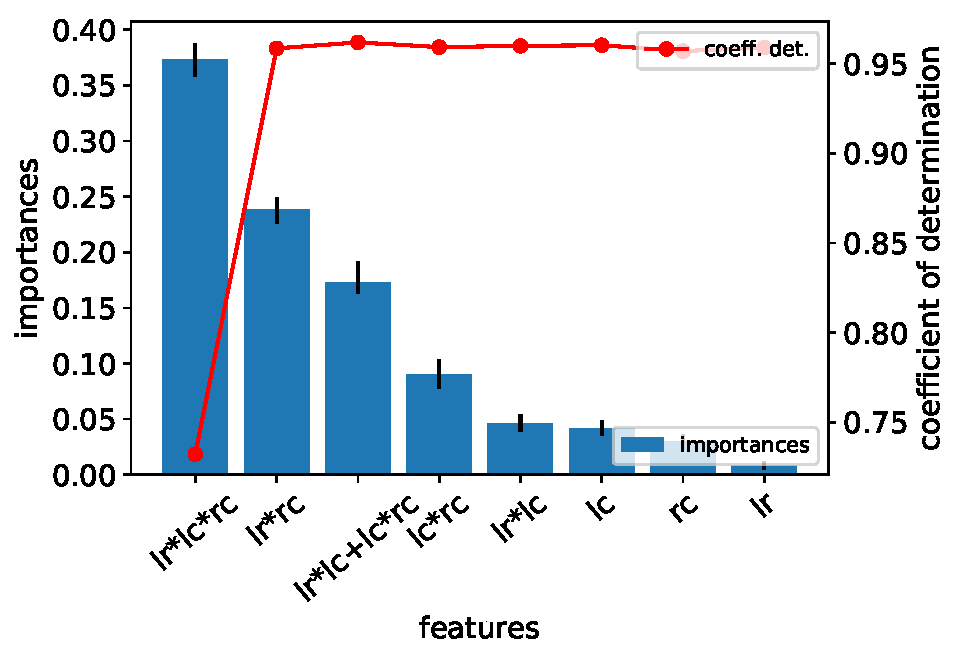
\includegraphics[width=0.45\textwidth]{figures/feature-importance.pdf}\caption{Relative importance of features and the impact on model accuracy. The number of multiplication operations, output matrix size, and  the shuffle overhead are the three most important features.}\label{fig:feature-importance}
\end{figure}

\subsubsection{Effectiveness of Bayesian optimization} The proposed MPEC uses Bayesian optimization to find optimal hyper-parameters for constructing a model. To analyze the influence of the optimization step quantitatively, we list three hyper-parameters and the $R^2$ value in Table~\ref{table:bo-performance}. In the experiments, we use the \textit{Bayesian optimization} library from the \textit{bayes\_opt} Python package. During optimization, we use 10-fold cross-validation to generate the training and test datasets and search for hyper-parameters to maximize $R^2$ over 30 iterations. Compared to the default parameters of the \textit{GB regressor}, the optimization step changes the model parameters to improve the accuracy, i.e., an increased number of regression trees (n\_estimators), while controlling overfitting, i.e., avoiding representing a case that is specific to a particular sample (min\_samples\_split). The final row of Table~\ref{table:bo-performance} summarizes that the accuracy of the model (as measured by the coefficient of determination) slightly increases from $0.9586$ to $0.9689$.

\begin{table}
  \centering
  \begin{tabular}{|C{2.2cm}|C{1.5cm}|C{1.5cm}|}
  \hline
  &Default&Bayesian optimization\\
  \hline
  n\_estimators&100&114\\
  \hline
  min\_samples\_split&2&14\\
  \hline
  max\_features&8&6\\
  \hline
  performance ($R^2$)&0.9586&0.9689\\
  \hline
  \end{tabular}
  \caption{\label{table:bo-performance}Parameters suggested by optimization module and the improved performance}
\end{table}

\subsubsection{Prediction algorithm comparison}
To predict the latency of matrix multiplication of various sizes and shapes, other machine learning algorithms can be applied with the proposed features. Among such algorithms, we compare a variant of decision tree regression algorithm and a linear regression variant method. For the decision tree variant, we compare \textit{GB regressor} (Section~\ref{sec:modeling}) and random forest~\cite{random-forest}. Unlike GB, the random forest regressor builds multiple regressor trees by randomly selecting features and samples. The GB and random forest regressors represent the non-linear characteristics of the input data while preventing overfitting by combining outcomes from many weak learners. For the linear regression variant, we adopt non-negative least squares (NNLS) regressor. When predicting latency, a non-negativity constraint is imposed to avoid latency being less than zero. The NNLS regressor finds the optimal linear model that minimizes the prediction error using this constraint.
% should be imposed to avoid the latency being less than zero. - unclear definition

Figure~\ref{fig:r2-comparison} shows the prediction accuracy of three algorithms. For each algorithm, we utilize the input dataset and features discussed in Section~\ref{sec:mpc-structure} and perform 10-fold cross-validation to split the training and test datasets. In total, 100 experiments are performed with different training and test datasets. The average value is plotted in Figure~\ref{fig:r2-comparison}, with the minimum and maximum values in error bars. As can be seen, the \textit{GB regressor} demonstrates the best accuracy with an $R^2$ value of $0.969$, followed by random forest regressor and NNLS, with  $R^2$ values of $0.955$ and $0.869$, respectively. Figure~\ref{fig:r2-comparison} also shows that the linear equation cannot capture the non-linear interactions among the features proposed herein. Figures~\ref{fig:gbm-measured-predicted} (\textit{GB regressor}) and \ref{fig:nnls-measured-predicted} (NNLS) show the measured and predicted latency in the x and y axes, respectively. Here, the dotted line indicates the prediction with no error (slope of one) and the scattered points close to the line represent accurate predictions. From the figures, we confirm that the \textit{GB regressor} provides better latency prediction accuracy.

% non-linear nonlinear?
\begin{figure}[t]
  \centering
  \subfloat[latency prediction accuracy]{\label{fig:r2-comparison}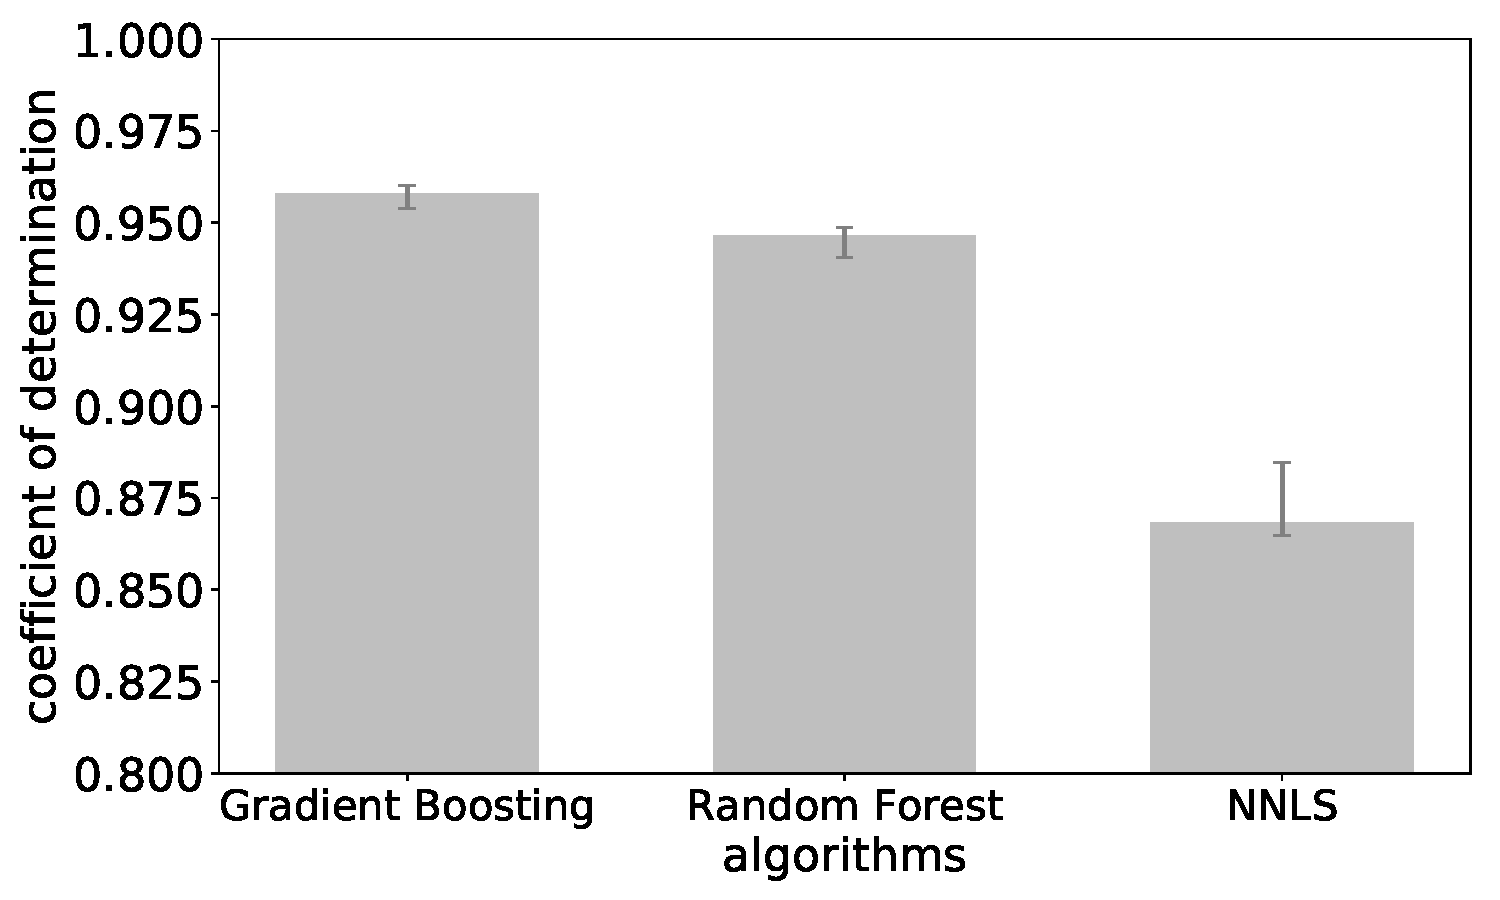
\includegraphics[width=0.4\textwidth]{figures/compare-algorithms.pdf}}\\
  \subfloat[gradient boosting regressor]{\label{fig:gbm-measured-predicted}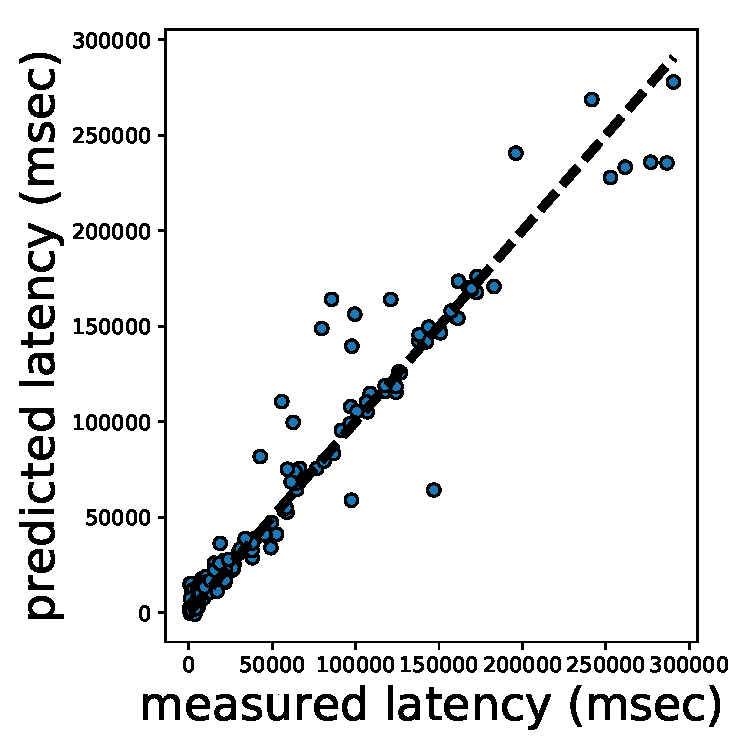
\includegraphics[width=0.23\textwidth]{figures/gbm-measured-predicted-1.pdf}} \hfil \subfloat[linear regressor]{\label{fig:nnls-measured-predicted}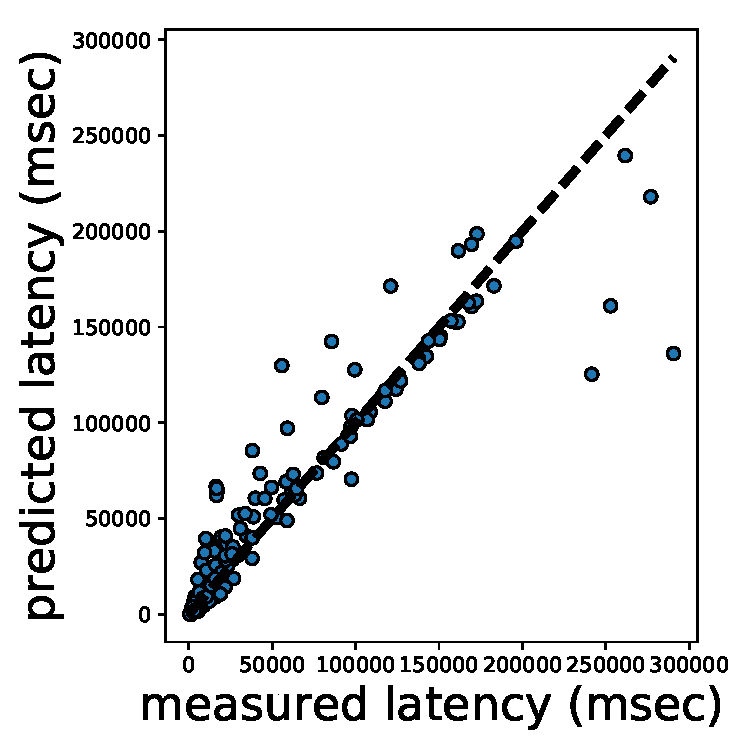
\includegraphics[width=0.23\textwidth]{figures/nnls-measured-predicted.pdf}}
  \caption{\label{fig:algorithm-comparison}Prediction accuracy comparison of various algorithms}
\end{figure}

\subsubsection{MPEC with various cloud computing instances}
To determine the applicability of the proposed MPEC on various cloud computing instances, we compare its performance using a compute-optimized EC2 instance (\textit{C4.2xlarge}), a GPU instance (\textit{G2.2xlarge}), and a memory-optimized instance (\textit{R4.2xlarge}). Despite having the same instance size (\textit{2xl}), different instances have distinct hardware configurations and hourly price. For example, the compute-optimized instance employs higher frequency processors with less RAM and the memory-optimized instance provides more RAM with a lower CPU frequency. Due to the different memory capacities of the instances, the maximum size of matrices for multiplication can differ. For a fair comparison, we select an intersection of matrix sizes that can be processed by all three instances. The input dataset generation and modeling steps are performed as discussed in Section~\ref{sec:mpc-structure}. For the model accuracy evaluation, 10-fold cross-validation is performed 100 times. The average $R^2$ value is shown in Figure~\ref{fig:gbm-diff-instances-r2-score} with error bars. As can be seen, regardless of instance type, the accuracy metric is greater than $0.9$. 
% higher lower -> needs comparsion, e.g., other than other instance types

To quantitatively understand the prediction accuracy of MPEC with different instance types, Figure~\ref{fig:gbm-measured-predicted-ticks} shows the latency of three representative workloads with different shapes, i.e., short-wide $\times$ long-thin, square $\times$ square, and long-thin $\times$ short-wide. For each workload, we calculate the measured latency (gray bar) and predicted latency (gray bar with dots) for each instance. Despite good prediction accuracy, the absolute latency value differs significantly among the different instances. For example, executing 128 $\times$ 5,000,000 $\times$ 128 matrix multiplication using the \textit{G2} instance involves three times greater latency compared with the \textit{R4} instance. If we consider the price of these two instances (as of writing), the \textit{R4.2xlarge} costs \$0.532 and the \textit{G2.2xlarge} instance costs \$0.65 in the us-west-2 region, the gap becomes even larger. These results demonstrate the importance of the accurate latency prediction of matrix multiplication in order to select appropriate cloud instances for big-data analysis workloads.
% For example, executing 128 $\times$ For example, caculating 128 $\times$
% neeeds comparison for the word "gap"

\begin{figure}[t]
	\centering
	\subfloat[latency prediction accuracy of different instance types]{\label{fig:gbm-diff-instances-r2-score}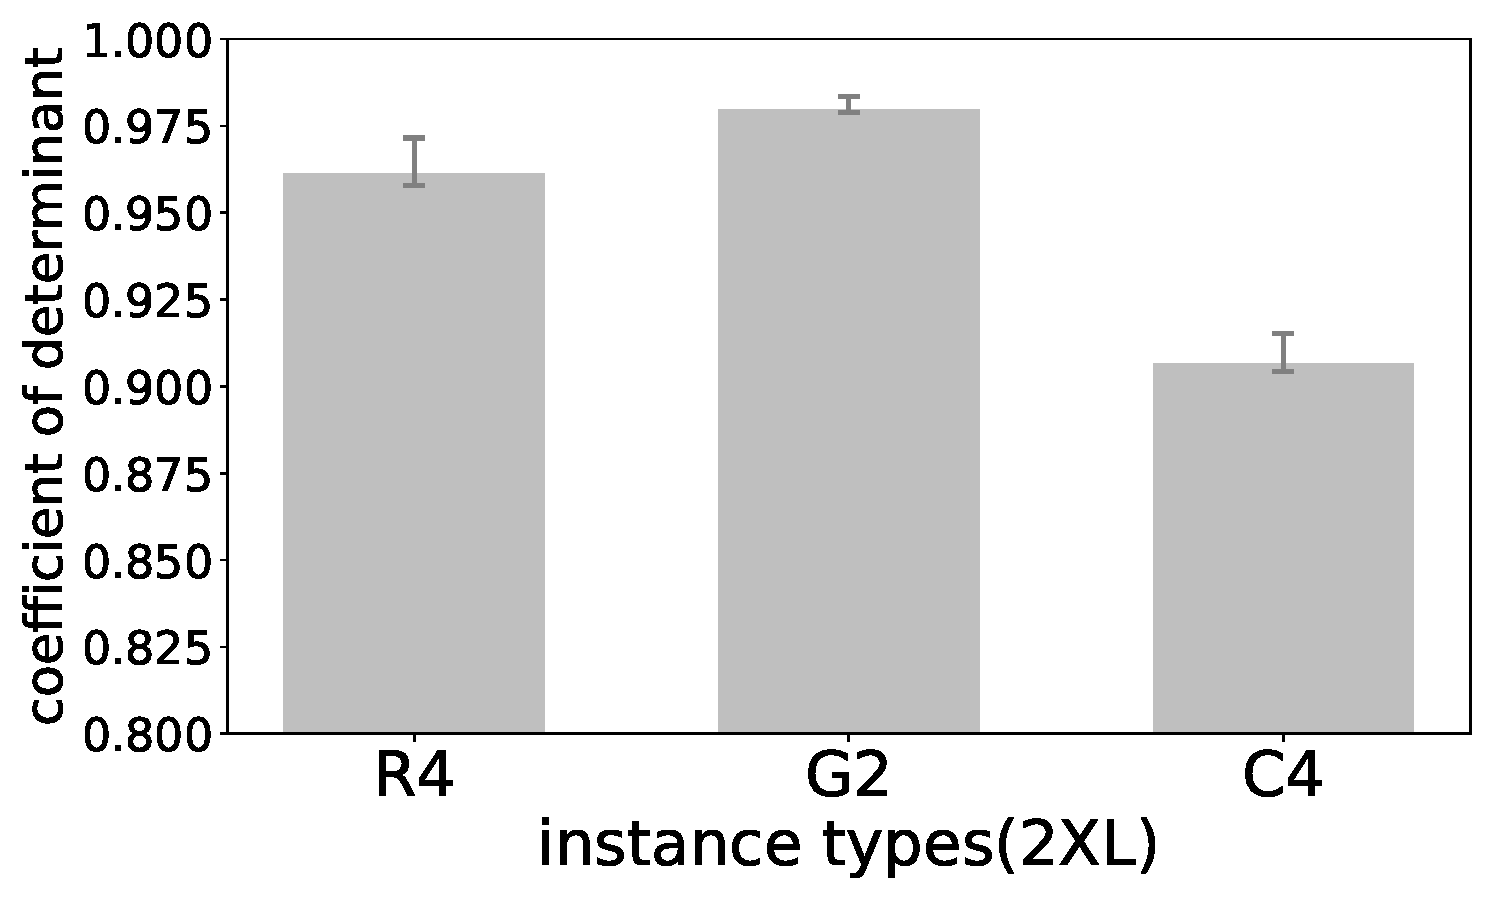
\includegraphics[width=0.4\textwidth]{figures/compare-instances-gbm-r2.pdf}}\\
	\subfloat[measured and predicted latency with different matrix shapes and instance types]{\label{fig:gbm-measured-predicted-ticks}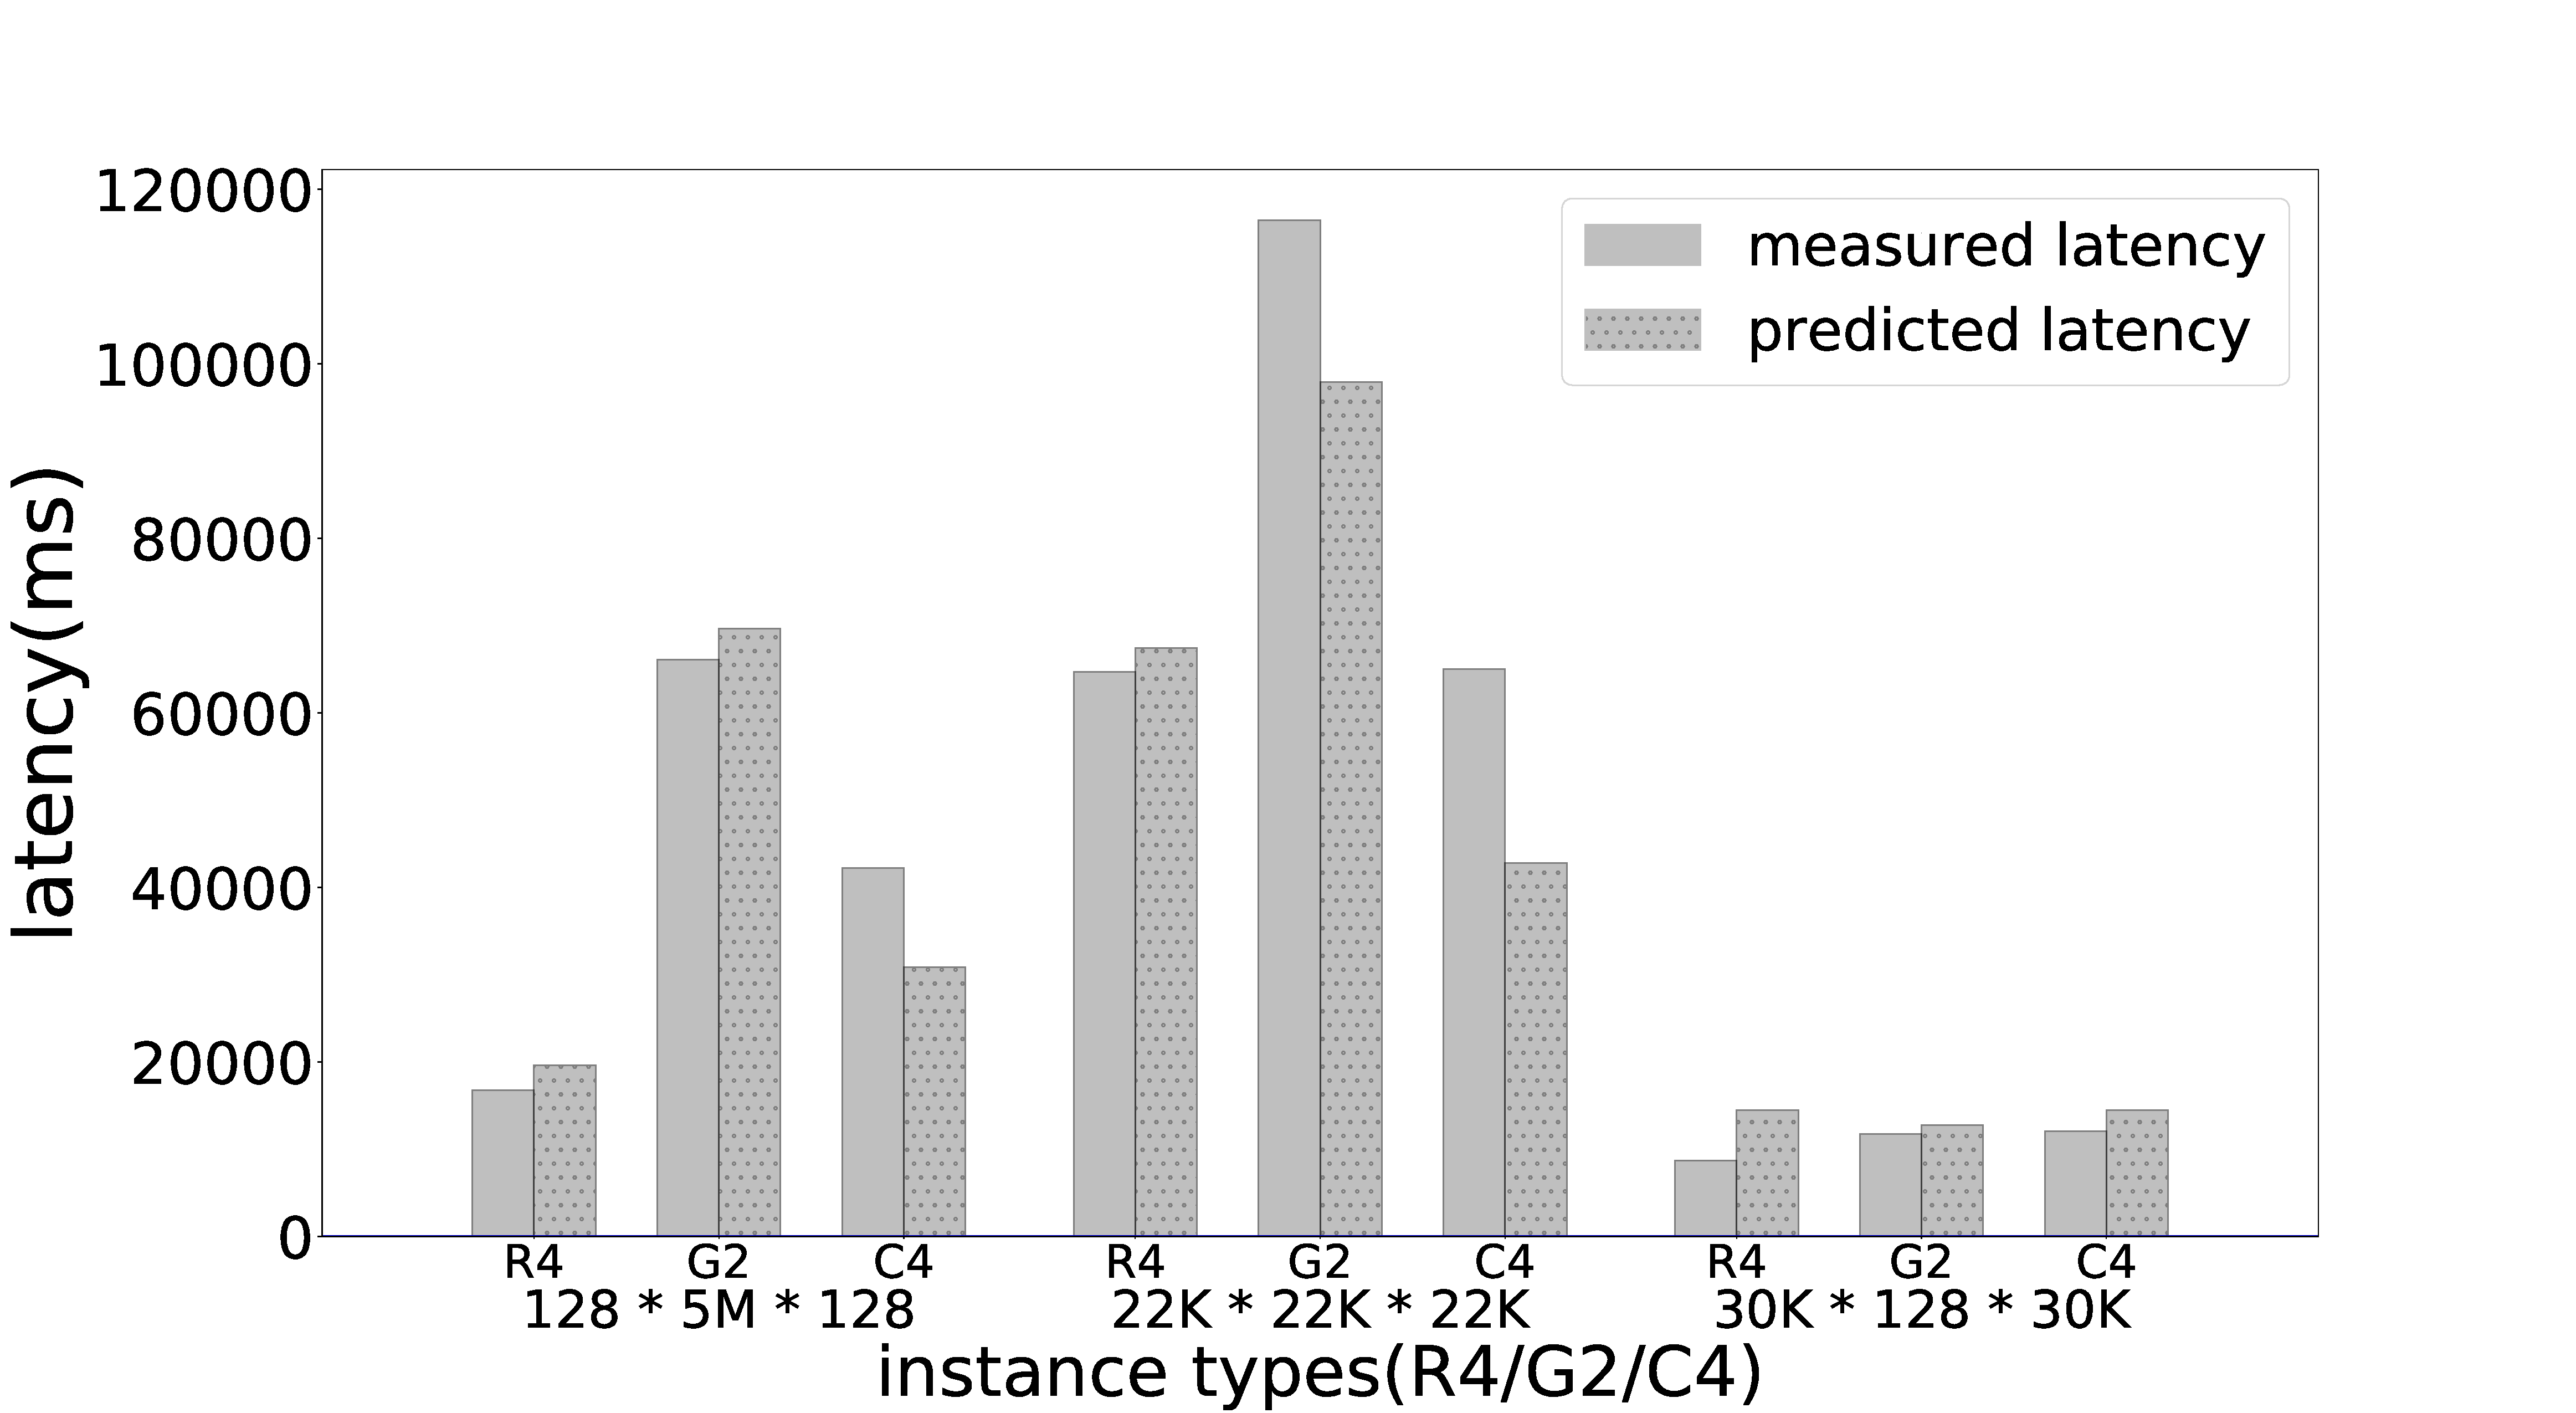
\includegraphics[width=0.5\textwidth]{figures/GBM-measured-predicted-ticks.pdf}} \hfil
	\caption{\label{fig:gbm-comparison}Performance of MPEC with different cloud computing instances}
\end{figure}

\subsubsection{Comparing MPEC to Ernest}
Ernest~\cite{ernest} is one of the most recent and accurate methods to provide cloud computing instance recommendation for various machine learning tasks. Ernest comprises two steps: experiment design and performance prediction. In the experiment design step, Ernest builds test cases using a small fraction of the sampled dataset and a distinct number of machines to run the experiments. In the prediction step, Ernest uses a linear regressor with the non-negativity constraint and metrics gathered from the experiments. To apply matrix multiplication tasks to Ernest, we should define the workload fraction to enable sampling; however, there is no clear way to scale down a matrix multiplication workload. Due to this limitation, we apply Ernest in two ways. First, we divide the number of elements (number of rows $\times$ number of columns) in the left and right matrices by the fraction, which we refer to as \textit{Ernest-Element}. The second way is to scale down the workload by the total number of multiplication operations (number of left matrix rows $\times$ left matrix columns $\times$ right matrix columns), which we refer to as \textit{Ernest-Multiply}. We select three representative matrix shapes, i.e., square $\times$ square, long-thin $\times$ short-wide, and short-wide $\times$ long-thin, with the largest matrix size available for execution with four \textit{R4.2xlarge} machines. While performing the Ernest experiments, some test cases could not be completed due to memory constraints, indicating Ernest's inaccuracy when generating test cases.

The experimental results are shown in Figure~\ref{fig:mpc-ernest}. For different matrix shapes, we show the true measured value, the predicted latency of MPEC, \textit{Ernest-Element}, and \textit{Ernest-Multiply}. Regardless of the workload scale-down mechanism, Ernest's prediction model shows poor accuracy in comparison with the proposed MPEC, except for the 128 $\times$ 8,000,000 $\times$ 128 workload. On average, the prediction accuracy of MPEC is better than that of the Ernest-Element and Ernest-Multiply by 28\% and 37\%, respectively. In addition to poor prediction accuracy, Ernest cannot reuse experimental results from other matrix multiplication tasks, because its experiment design requires scaling down the original workloads precisely by the dataset fraction and number of machines. In contrast, the proposed MPEC can reuse the results of other matrix multiplication tasks to increase the size of the input dataset pool, thereby improving the model accuracy using more diverse matrix multiplication scenarios.

\begin{figure}[t]
	\centering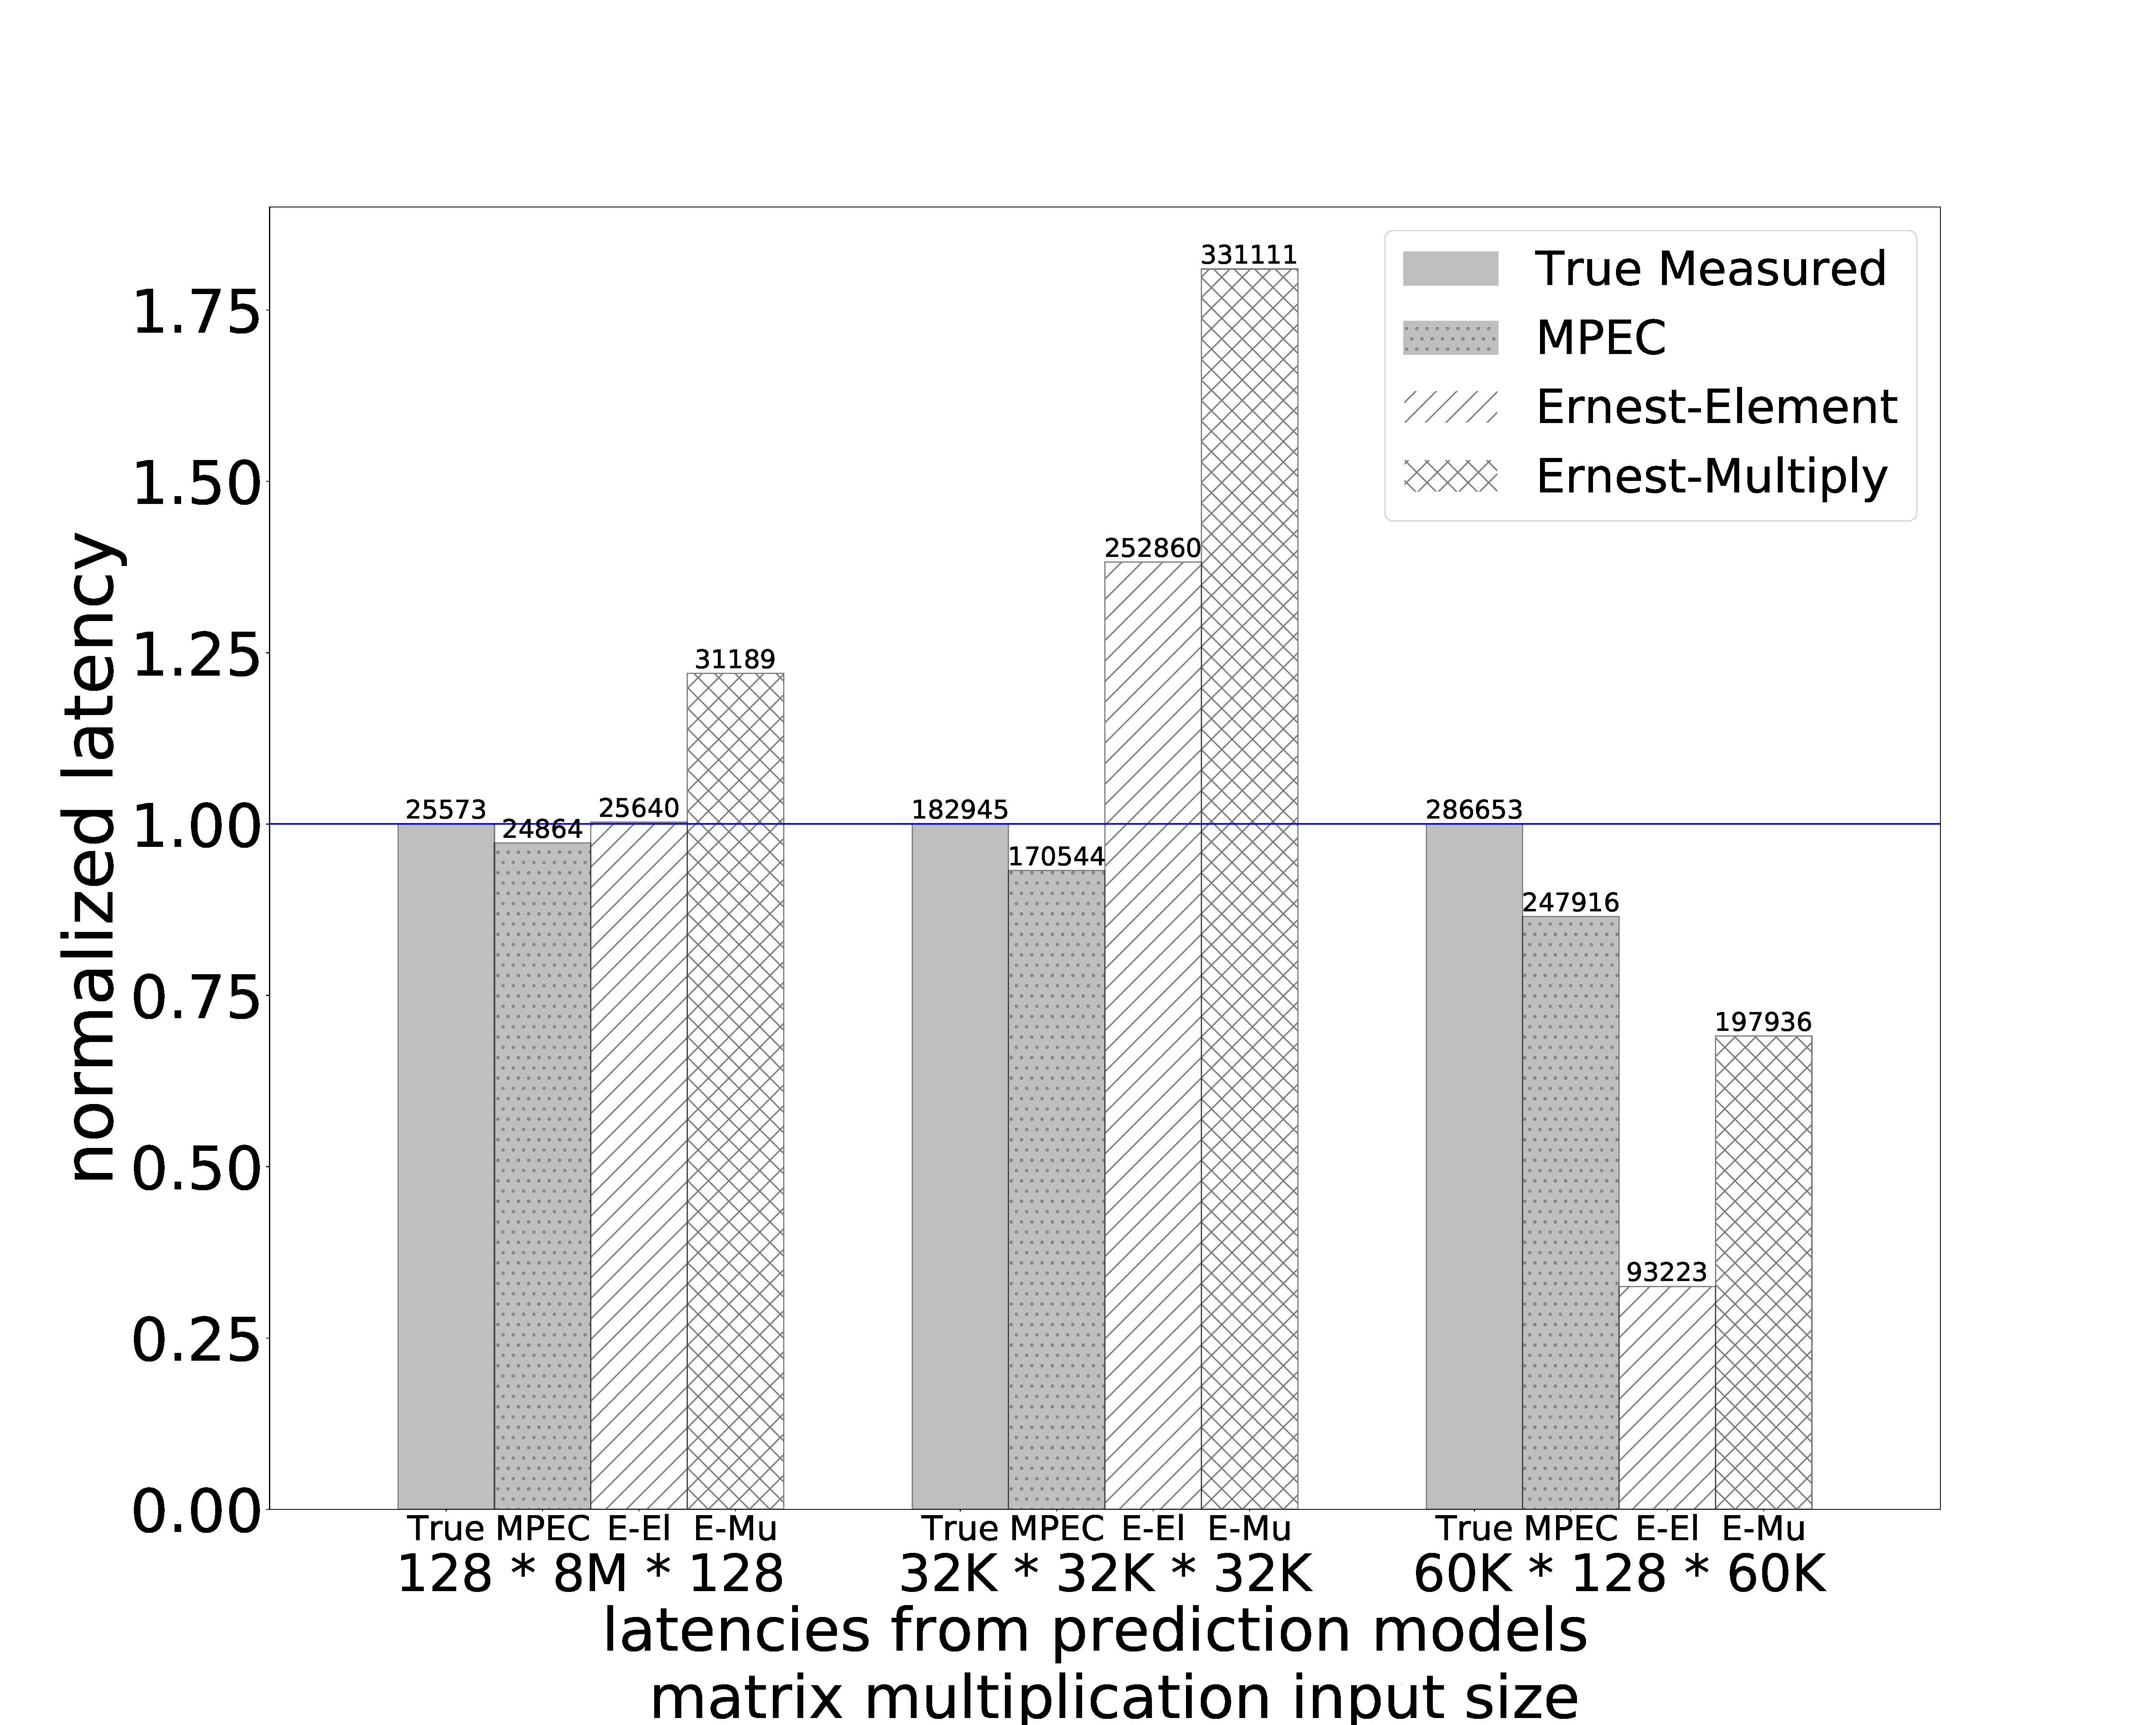
\includegraphics[width=0.5\textwidth]{figures/MPC-Ernest-compare.pdf}\caption{Comparison of MPEC with Ernest}\label{fig:mpc-ernest}
\end{figure}

\section{Related Work}\label{sec:relatedwork}
\textbf{Big data workload performance estimation on cloud}: In a cloud computing environment, there are many instance types with unique hardware configurations. Few studies have proposed methods to build an optimal environment for dealing with big data analysis workloads. Ernest~\cite{ernest} employs an algorithm that predicts the performance of arbitrary data mining algorithms with different numbers of workers in the cloud. PARIS~\cite{paris} follows a hybrid online/offline approach, where a random forest model is used to predict the application performance under various VM configurations based on features such as CPU utilization obtained from profiling. CherryPick~\cite{cherrypick} uses Bayesian optimization to select instance type candidates for offline profiling in order to predict performance on various cloud instance types. These approaches rely on a scale-based sampling method for a given input dataset, and the profiled result is not reusable for other input datasets. Furthermore, they focus on predicting high-level machine learning algorithm execution latency and cannot capture the complex nature of a distributed matrix multiplication task. Thus, their prediction accuracy is reduced when they are applied to an algorithm whose kernel is distributed matrix multiplication.

FiM~\cite{fim} estimates the running time of iterative and multistage cloud-based HPC applications by modeling the status of CPU cycles using a stochastic Markov model with linear regression to estimate the parameters of the model. Similar to FiM, Mariani et al.~\cite{hpc-cloud-predict} proposes a machine-learning based modeling method to predict HPC application performance in the cloud. Their method first profiles the behavior of an application using hardware-independent metrics and then runs the application on a few cloud instances to measure the performance. The correlation between application metrics and the cloud instance is discovered using the random forest algorithm. These two methods rely on the sampling of the applications or the input dataset, and their models are not reusable for a new dataset. In MPEC, we measure the latency of the matrix multiplication tasks of arbitrary sizes and the previous experimental results can be used to improve the prediction accuracy of any input.

\textbf{Optimizing cloud-based distributed matrix multiplication}: Matrix multiplication is an important task in machine learning jobs with large-scale datasets. Due to the importance of the task and the ever-increasing sizes of datasets, many studies have focused on optimizing the task in a distributed cloud computing environment. Yu et al.~\cite{matmult-overhead-profiling} thoroughly investigates the communication overhead of various distributed matrix multiplication shapes and proposes a task execution plan to minimize the communication cost. Marlin~\cite{marlin} proposes a distributed matrix multiplication algorithm on Spark to minimize the shuffle overhead. As discussed quantitatively in this study, shuffle overhead is crucial for determining the performance of distributed matrix multiplication tasks; however, other than the shuffle overhead, the output matrix size and total number of product operations also impose significant impact on overall task completion time.

\section{Conclusion and Future Work}
In this paper, we propose MPEC, a method for predicting the execution time of distributed matrix multiplication with various input datasets on a variety of cloud computing instances. We first characterize the overheads of distributed matrix multiplication and propose eight features that represent different steps of the task. In the modeling step, we employ a GB regressor to model non-linear interactions among the features and Bayesian optimization to find better performing hyper-parameters in an efficient manner. We evaluated more than 200 cases of various matrix multiplication scenarios (e.g., square $\times$ square, long-thin $\times$ short-wide, and short-wide $\times$ long-thin) on various cloud computing instances. The evaluation results reveal that among the proposed features, the number of product operations, the output matrix size, and shuffle overhead are the three most important features that determine the overall latency. A performance comparison with the state-of-the-art cloud computing performance predictor Ernest reveals that the proposed MPEC provides 16\% more accurate results when predicting the latency of a distributed matrix multiplication task.

We are currently working on selecting a small number of representative distributed matrix multiplication workloads that provide high prediction accuracy while reducing the performance profiling overhead on different cloud computing instances. In addition to the proposed features for modeling task latency with MPEC, we plan to add additional features of unique cloud computing instance configurations, e.g., clock rate, network bandwidth, and memory size. We expect that these additional features will help to predict the task latency of different types of cloud computing instances.
\bibliographystyle{IEEEtranS}
\bibliography{abc2}
\end{document}
